\documentclass[11pt]{article}
\usepackage{amsmath,amsthm,amssymb,fullpage,graphicx,hyperref,listings}
\author{Andy Reagan}
\title{Math 337 Homework 03}

     \def\NN{\mathbb{N} }
     \def\ZZ{\mathbb{Z} }
     \def\QQ{\mathbb{Q} }
     \def\RR{\mathbb{R} }
     \def\CC{\mathbb{C} }
     \def\f{\frac }
     \def\b{\begin }
     \def\e{\end }
     \def\Log{\text{Log} \,}
     \def\Re{\text{Re} \, }

\begin{document}
\maketitle

\begin{enumerate}

\item Using Taylor expansions of $y'_{i-1}$ and $y'_{i-2}$ about $x = x_i$, verify that
\[ y_i ''' = \f{y_i'-2y_{i-1}'+y_{i-2}'}{h^2} + O(h) . \]

\bigskip
\textbf{Solution:} From Equation 3.10 we have that
\[ y_{i} '' = \f{y_i'-y_{i-1}'}{h} +O(h).\]
Taking the derivative of this we have
\[ y_{i} ''' = \f{y_i''-y_{i-1}''}{h} .\]
Putting equation 3.10 into the above, we have
\[ y_{i} ''' = \f{\f{y_i'-y_{i-1}'}{h} +O(h) -\left (\f{y_{i-1}'-y_{i-2}'}{h} +O(h) \right )}{h} = \f{yi'-2y_{i-1}'+y_{i-2}'}{h^2} + O(h), \]
as desired.

\item Obtain the counterpart of the linear system in Equation 3.15 {\emph without} assuming that $x_i = 0.$

\bigskip
\textbf{Solution:} Without making that assumption, we have the system of equations
\begin{align} f = 1 \Rightarrow & \int _{x_i} ^{x_{i+1}} 1\,dx = h \cdot (b_0 \cdot 1 + b_1 \cdot 1 + b_2 \cdot 1 )\\
f = x \Rightarrow & \int _{x_i} ^{x_{i+1}} x\,dx = h \cdot (b_0 \cdot x_i + b_1 \cdot(x_i-h) + b_2 \cdot (x_i - 2h ))\\
f = x^2 \Rightarrow & \int _{x_i} ^{x_{i+1}} x^2\,dx = h \cdot (b_0 \cdot x_i^2 + b_1 \cdot(x_i-h)^2 + b_2 \cdot (x_i - 2h )^2)\end{align}
Solving both the integrals and expanding the RHS, this system becomes
\begin{align} & h = h b_0 + h b_1 + h b_2\\
& x_ih + \f{h^2}{2} = h b_0 x_i + h b_1 x_i-h^2 b_1+ h b_2 x_i - 2 b_2 h^2\\
& x_i^2 h + h^2 x_i + \f{h^3}{3} = h b_0 x_i^2 + hb_1 x_i^2 - 2b_1x_i h^2 +b_1h^3 + b_2 x_i^2 h - 4 b_2 h^2 x_i + 4b_2 h^3\end{align}
We begin solving this system of three equations and three unknowns by diving by $h$ in Equation 4 to obtain
\begin{equation} 1 = b_0 + b_1 + b_2 \end{equation}
and grouping the $hx_i$ terms in Equation 5 for
\begin{equation}  \f{h^2}{2} + x_ih = h x_i( b_0 + b_1+  b_2) -h^2( b_1 + 2 b_2). \end{equation}
Using Equation 7 in the above Equation 8, we cancel and divide by $h^2$ to obtain
\begin{equation}  -\f{1}{2} = 2 b_2 + b_1 ~~ \Rightarrow ~~b_1 = -2b_2 -\f{1}{2}. \end{equation}
Similarly, we group terms in $x_i^2h$ and $h^2x_i$ in Equation 6, using Equation 7 and 9 to cancel them, repspectively, and grouping by powers of $h^3$ are left with
\begin{equation} h^3(\f{1}{3} - b_1+4b_2 ) =  0. \end{equation}
We stop here, having arrived at precisely the form of Equations 3.15 (7,9 and 10 here).

\item Find the coefficients $b_{-1},b_0,b_1$ in
\[ Y_{i+1}  = Y_i + h (b_{-1} f_{i+1} + b_0 f_i + b_1 f_{i-1}) \]
that produce a 3-rd order method.

\bigskip
\textbf{Solution:} Following the derivation in Section 3.2, I approximate the solution as the integral of $f$, and require the coefficients to create a method that is exact for a third degree polynomial, $y = p_3$.
Therefore, we represent $f$ as a second-degree polynomial $p_2$ have solve the system 
\begin{align} f = 1 \Rightarrow & \int _0 ^h 1\,dx = h \cdot (b_{-1} \cdot 1 + b_{0} \cdot 1 + b_{1} \cdot 1 )\\
f = x \Rightarrow & \int _{0} ^{h} x\,dx = h \cdot (b_{-1} \cdot (x_i+h) + b_{0} \cdot x_i + b_{1} \cdot (x_i - h ))\\
f = x^2 \Rightarrow & \int _{0} ^{h} x^2\,dx = h \cdot (b_{-1} \cdot (x_i+h)^2 + b_{0} \cdot(x_i)^2 + b_{1} \cdot (x_i - h )^2)\end{align}
Equation 11 is the same form as Equation 6 in Problem 2, and so we have a similar result reducing this.
Using the assumption that $x_i = 0$ in the Equations 12 and 13 leaves us with the two equations:
\begin{align} & h^2/2  = h \cdot (b_{-1} h - b_{1} h )\\
& h^3/3 = h \cdot (b_{-1} h^2  + b_{1} h ^2)\end{align}
Cancelling the $h$ terms in the above two equations, we substitue to find $b_1,b_{-1}$ and use Equation 6 to obtain $b_0$.
We find
\begin{equation} b_{1} = 5/12, b_0 = 2/3, ~\text{and}~ b_{-1} = -1/12 .\end{equation}

\item Use the Predictor-Corrector method given by Eqs 3.33, 3.39, and 3.40 to solve
\begin{equation} y' = \sin y, ~~~~ y(0) = 1, ~~~~ x \in [0, \pi ] . \end{equation}
Select the step size so that the local truncation error, given by 3.39, be at most $\epsilon _{\text{loc}} = 10^{-4}$.
Provide an  explanation for your choice of the step size.

\bigskip
\textbf{Solution:} First note that using separation of variables, the analytical solution to the ODE given above is
\begin{equation} y(t) = 2 * \text{cot} ^{-1} \left ( e^{-t} \text{cot} (1/2) \right ).\end{equation}

Using formula 1.28, the third derivative of $y$ is
\begin{equation} y'''(x) = -8\sin(x)\cos(x) -2\sin^2(x)\cos^4(x) -6\sin^2(x)\cos(x) .\end{equation}
With the error given by Equation 3.39, we compute $h$ for $\epsilon _\text{loc} = 10^{-4}$ and choose the max of $y'''(x)$ on $[0,\pi]$.

Figure 1 is a plot of $y'''$, with the max as a big square. We use the maximum to compute the timestep. In Figure 2, we plot the numerical solution and the analytical solution. We test whether our timestep controlled the error in Figure 3.
Figure 4 gives us an idea of the improvement of Equation 3.40 over Equations 3.33, by plotting the difference in true error of $Y_p$ and $Y_{i+1}$.
We see that the error estimate which we made was sufficient to contain the error within $\epsilon _\text{loc} = 10 ^{-4}$.

All of these figures are created, saved, and closed individually in the script \verb!andy_hw03_prb4.m!.
The step size computation, shown in the code, is equivalent to solving 3.37 with our estimate of $y'''$ given above:

\[ |\epsilon_{i+1} | \approx 1/12 \cdot h^3 | y''' _{i+1}| ~~~~~~~~~\Rightarrow~~~~~~~~ h \approx \sqrt[3]{12 |\epsilon_{\text{loc}}| / | y''' _{i+1}|} .\]

I also plot and save the improvement of Equation 3.40 over 3.35, that is, the difference in the actual error of each method.
Looking at the code, I took care to make the plots in the a loop.
I also loop over the initialization method, using a Modified Euler method for second order accuracy and Kutta's third order method for third order accuracy.
To see the results for the ME start, run the code.
Here, for brevity, I just include the results starting with RK3.

\pagebreak
\lstinputlisting[language=Matlab]{andy_hw03_prb4.m}

\pagebreak

\begin{figure}[h!]
  \centering
  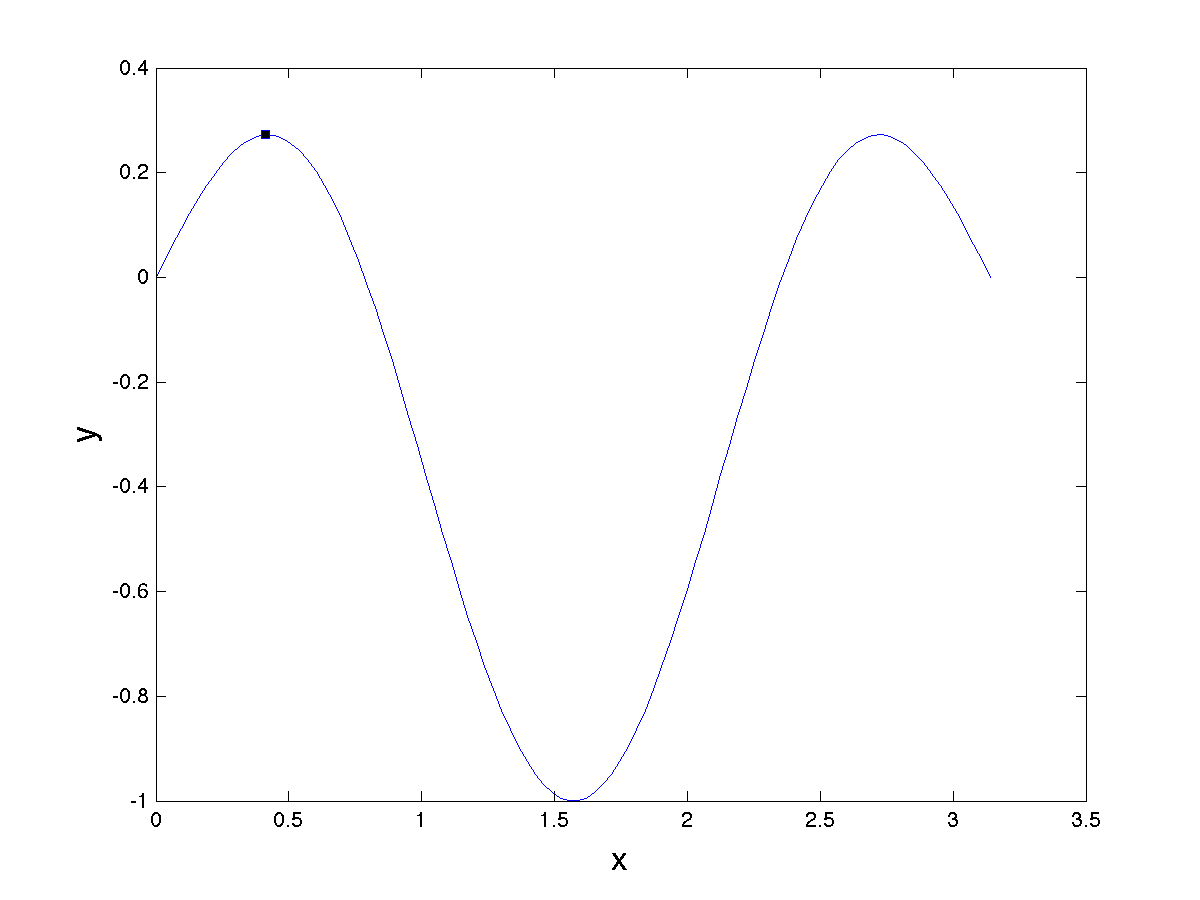
\includegraphics[width=0.8\textwidth]{andy_hw03_prb4_ytp.png}
  \caption{A plot of $y'''$. The max is labeled by the black box.}
\end{figure}

\begin{figure}[h!]
  \centering
    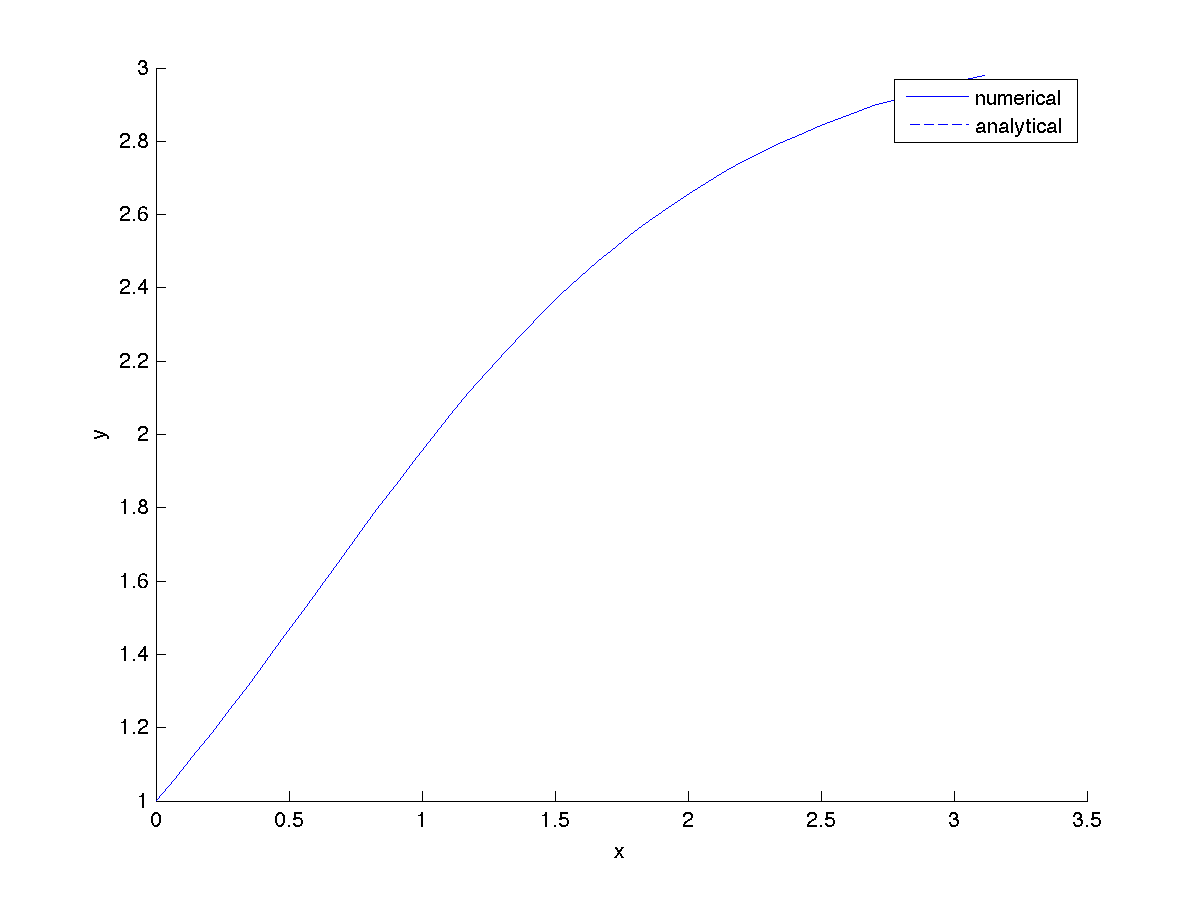
\includegraphics[width=0.8\textwidth]{andy_hw03_prb4_RK3_both.png}
  \caption{The numerical, and analytical, solution. They are so close that it is difficult to tell them apart.}
\end{figure}

\begin{figure}[h!]
  \centering
    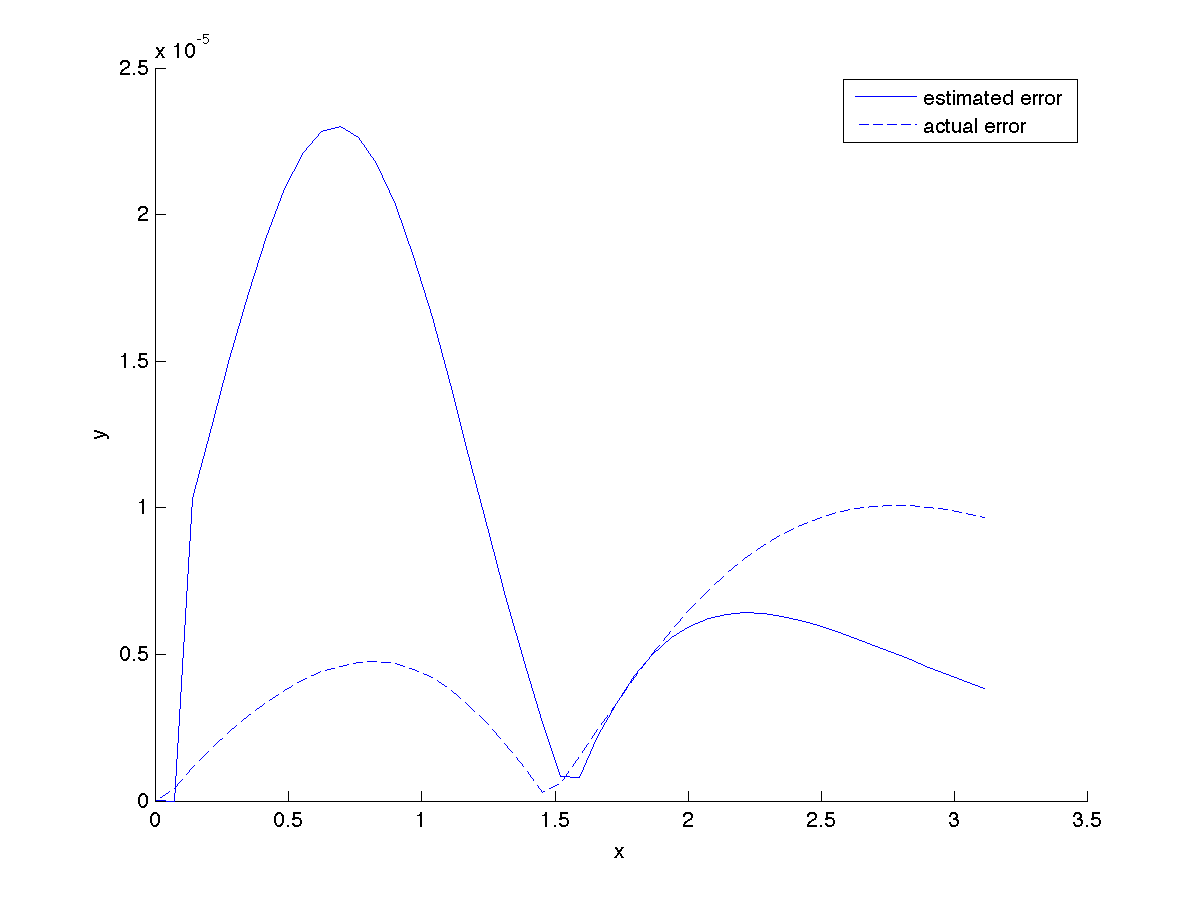
\includegraphics[width=0.8\textwidth]{andy_hw03_prb4_RK3_error_both.png}
  \caption{The estimated (dashed) and true error at each timestep of the integration.}
\end{figure}

\begin{figure}[h!]
  \centering
    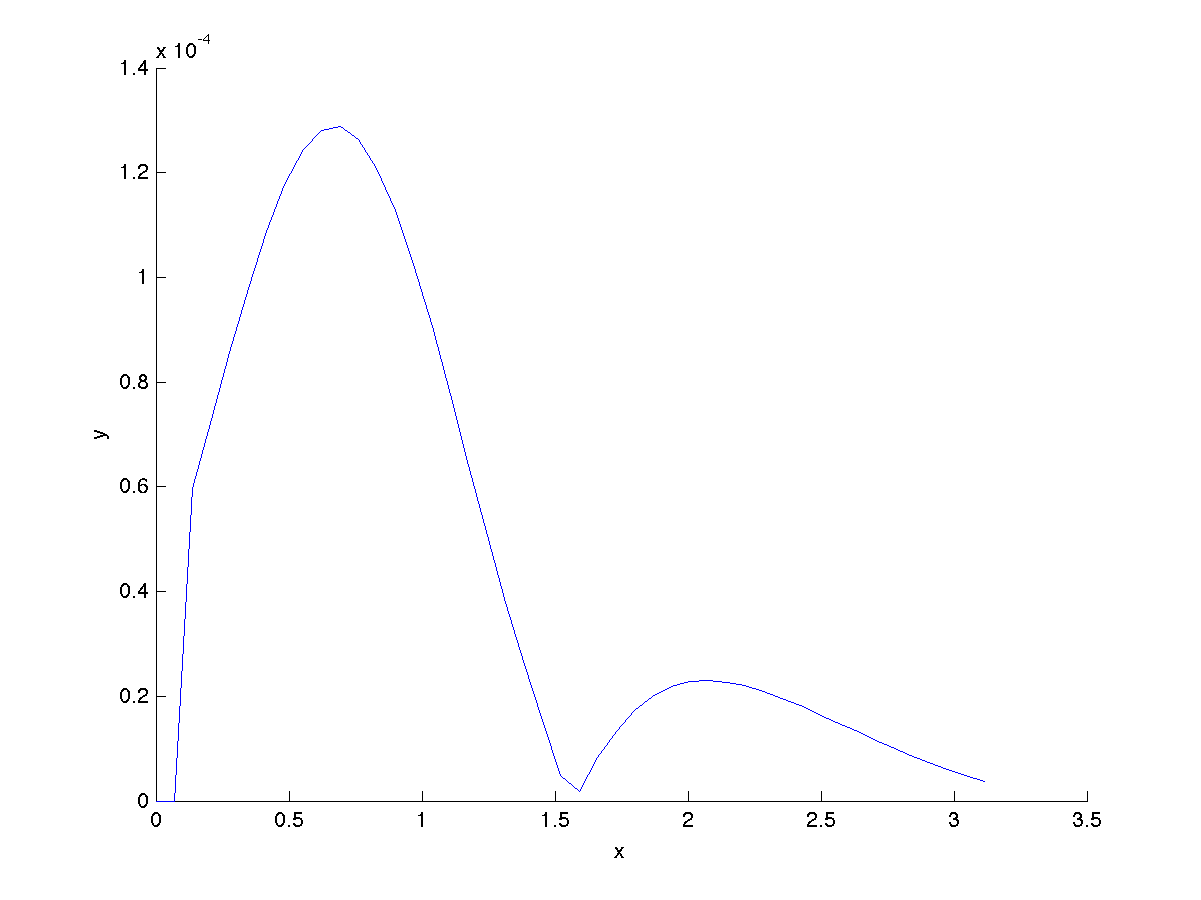
\includegraphics[width=0.8\textwidth]{andy_hw03_prb4_RK3_improvement.png}
  \caption{The improvement of Equation 3.40 over Equations 3.33, by plotting the difference in true error of $Y_p$ and $Y_{i+1}$.}
\end{figure}


\end{enumerate}



\end{document}
